\chapter{Detail Design}

\section{Transistor Switch}

\begin{figure}[h]
\centering
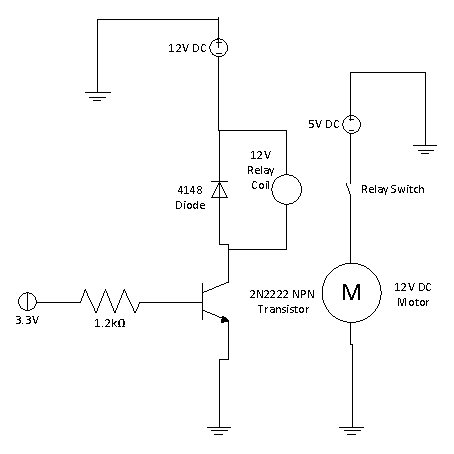
\includegraphics[scale=0.7]{relay_switch.eps}
\caption{12V relay transistor switch. }
\end{figure}

\section{server program}
\subsection{nfc}
\subsection{qr code}

\section{vending program}
\subsection{nfc}

Because the Arduino version of this shield is locally available, and the cost issues related
to importing a NFC chip that is made for the Raspberry Pi, the Arduino version was bought for 
R780.00. Its Transistor-Transistor Logic (TTL) serial interface was configured in such a way
so that it can serially communicate with the Raspberry Pi's UART interface. It can be powered
by the 5V output pin from the Raspberry Pi. 

\subsection{qr code}

\section{Android app}

\section{Motor and coil}